\documentclass[a4paper,12pt]{article}
% --- 日本語とフォント設定(LuaLaTeX専用) ---
\usepackage{luatexja}
\usepackage{luatexja-fontspec}
\setmainfont{TeX Gyre Termes}    % 欧文フォント
\setmainjfont{HaranoAjiMincho}       % 和文フォント

\setlength{\headheight}{15pt}

% --- ページレイアウト ---
\usepackage[top=30truemm,bottom=30truemm,left=25truemm,right=25truemm]{geometry}

% --- パッケージ ---
\usepackage{pdfpages}
\usepackage{graphicx}
\usepackage{amsmath,amssymb}
\usepackage{fancyhdr}
\usepackage{listings}
\usepackage{color}
\usepackage{caption}
\usepackage{titlesec}
\usepackage{cite}
\usepackage{animate}
\usepackage{subcaption}
\usepackage{float}
\usepackage{array}
\usepackage{multirow}
\usepackage{longtable}
\usepackage{xcolor}
\usepackage{booktabs}
\usepackage{siunitx}
\usepackage{url}
\usepackage{chngcntr}
\usepackage{multicol}

\makeatletter
\newenvironment{tablehere}
  {\def\@captype{table}}
  {}

\newenvironment{figurehere}
  {\def\@captype{figure}}
  {}
\makeatother
% 全体のページ設定
 
% ページ番号をフッタにふる
\setlength{\columnsep}{10mm}
\columnseprule=0.2mm
\pagestyle{plain}
 
\makeatletter
 
\def\@thesis{}
\def\id#1{\def\@id{#1}}
\def\master#1{\def\@master{#1}}
\def\department#1{\def\@department{#1}}
 
\def\@maketitle{
\begin{center}
{\huge \@thesis \par} %修士論文と記載される部分
\vspace{5mm}
{\LARGE\bf \@title \par}% 論文のタイトル部分
\vspace{5mm}
{\Large 提出日 \@date\par} % 提出年月日部分
\vspace{5mm}



{\Large 氏名 \@author}% 氏名
\end{center}
%\par\vskip 1.5em
 
}
 
\makeatother
 
\title{第3回輪講資料}
\date{\today}
\author{4315 世田直己馳}
 
% ここから本文内容記載する
 
\begin{document}

% 表紙を表示させる
 
\maketitle
% 改ページ

\begin{multicols}{2}
\section{はじめに}
ゼミ課題の光を使った通信の進捗について報告する。

\section{各自の進捗}
各自の進捗報告を図\ref{sintyoku}に示す。
\begin{figure}[H]
  \centering
  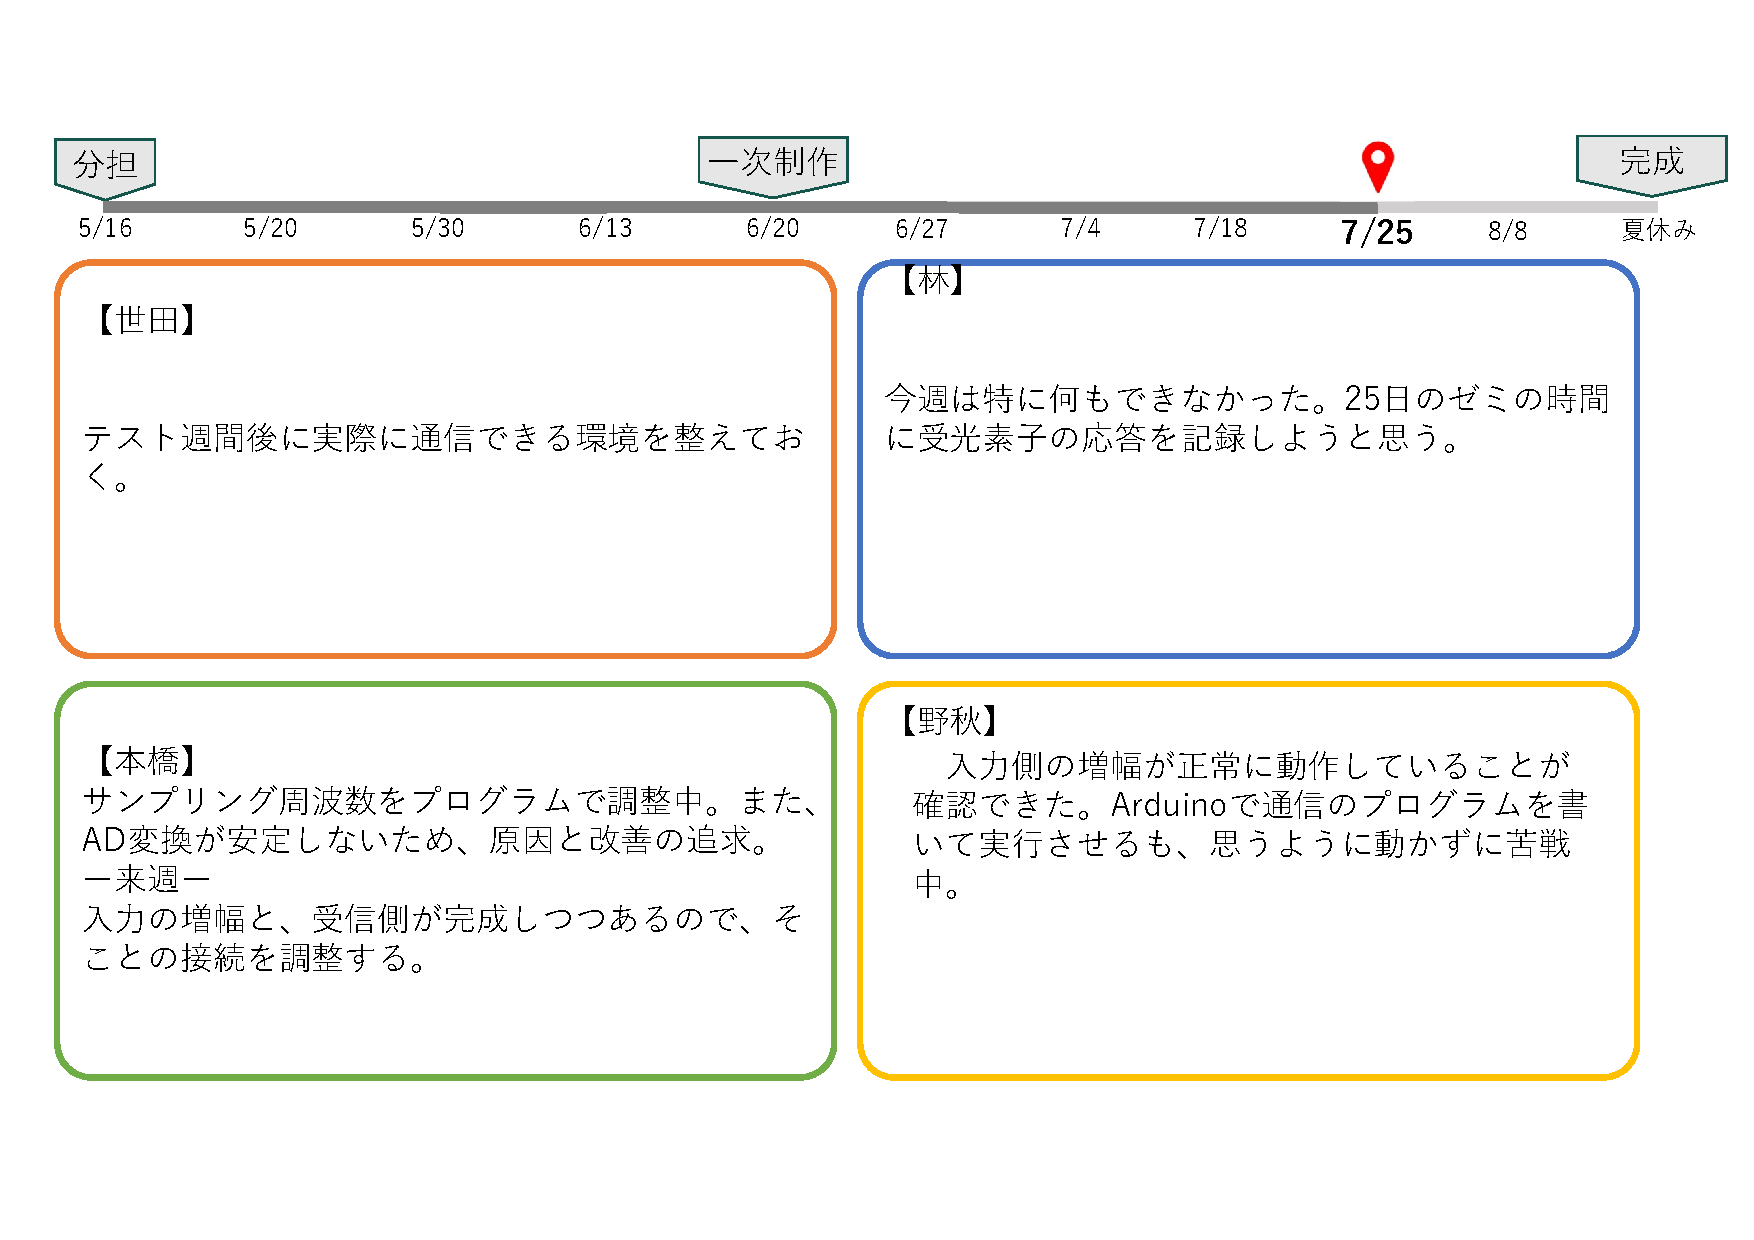
\includegraphics[width=0.4\textwidth]{fig/sintyoku.pdf}
  \caption{各自の進捗報告}
  \label{sintyoku}
  \end{figure}

\section{受講部の作成}
作成した受講部の回路図を図\ref{jukou}に示す。

\begin{figure}[H]
  \centering
  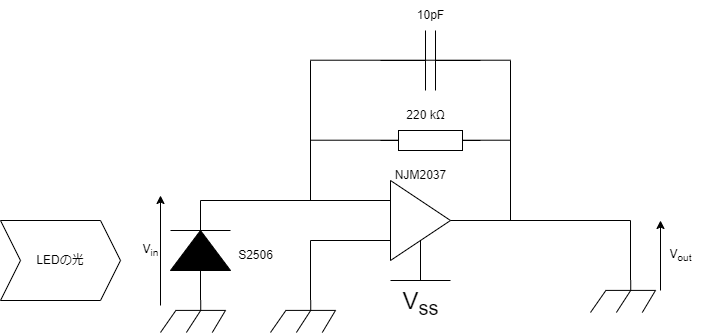
\includegraphics[width=0.4\textwidth]{fig/LEDjukou.png}
  \caption{LED受講部の回路図}
  \label{jukou}
  \end{figure}

  得られた信号を図\ref{jukou2},図\ref{jukou3}に示す。
  \begin{figure}[H]
    \centering
    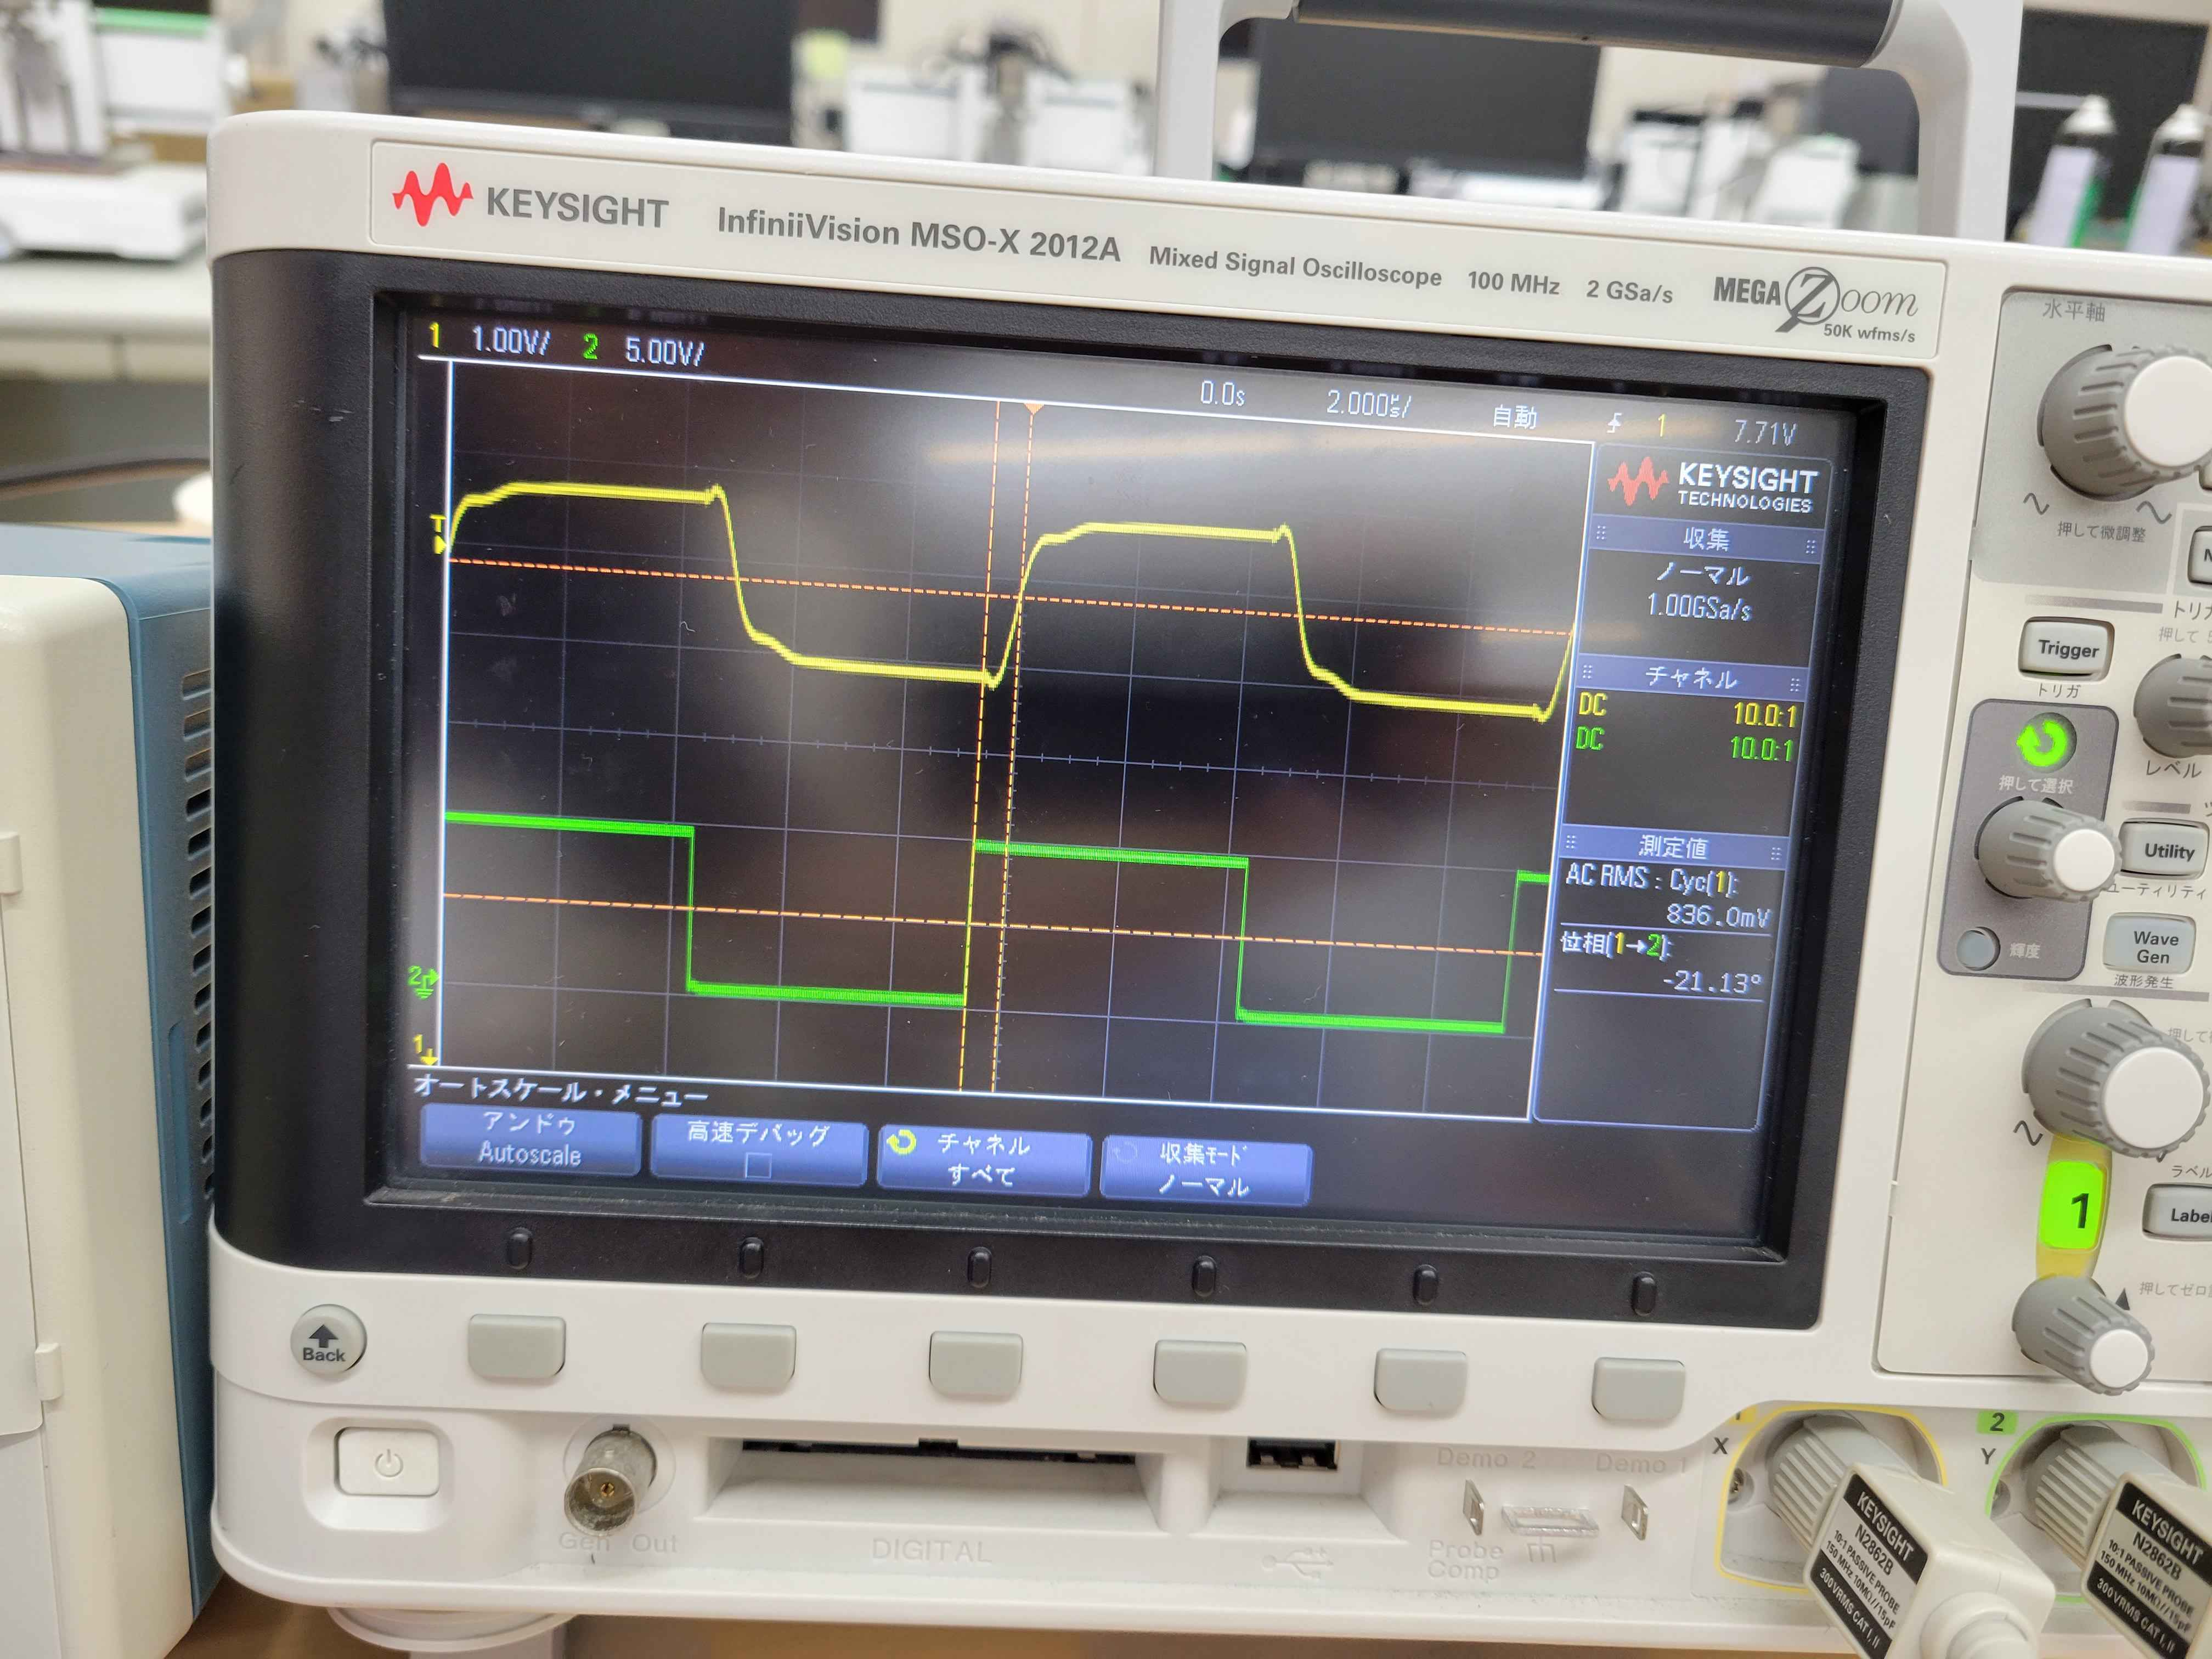
\includegraphics[width=0.4\textwidth]{fig/100.jpg}
    \caption{100 kHzの信号でLEDを光らせた時の波形}
    \label{jukou2}
    \end{figure}
    \begin{figure}[H]
      \centering
      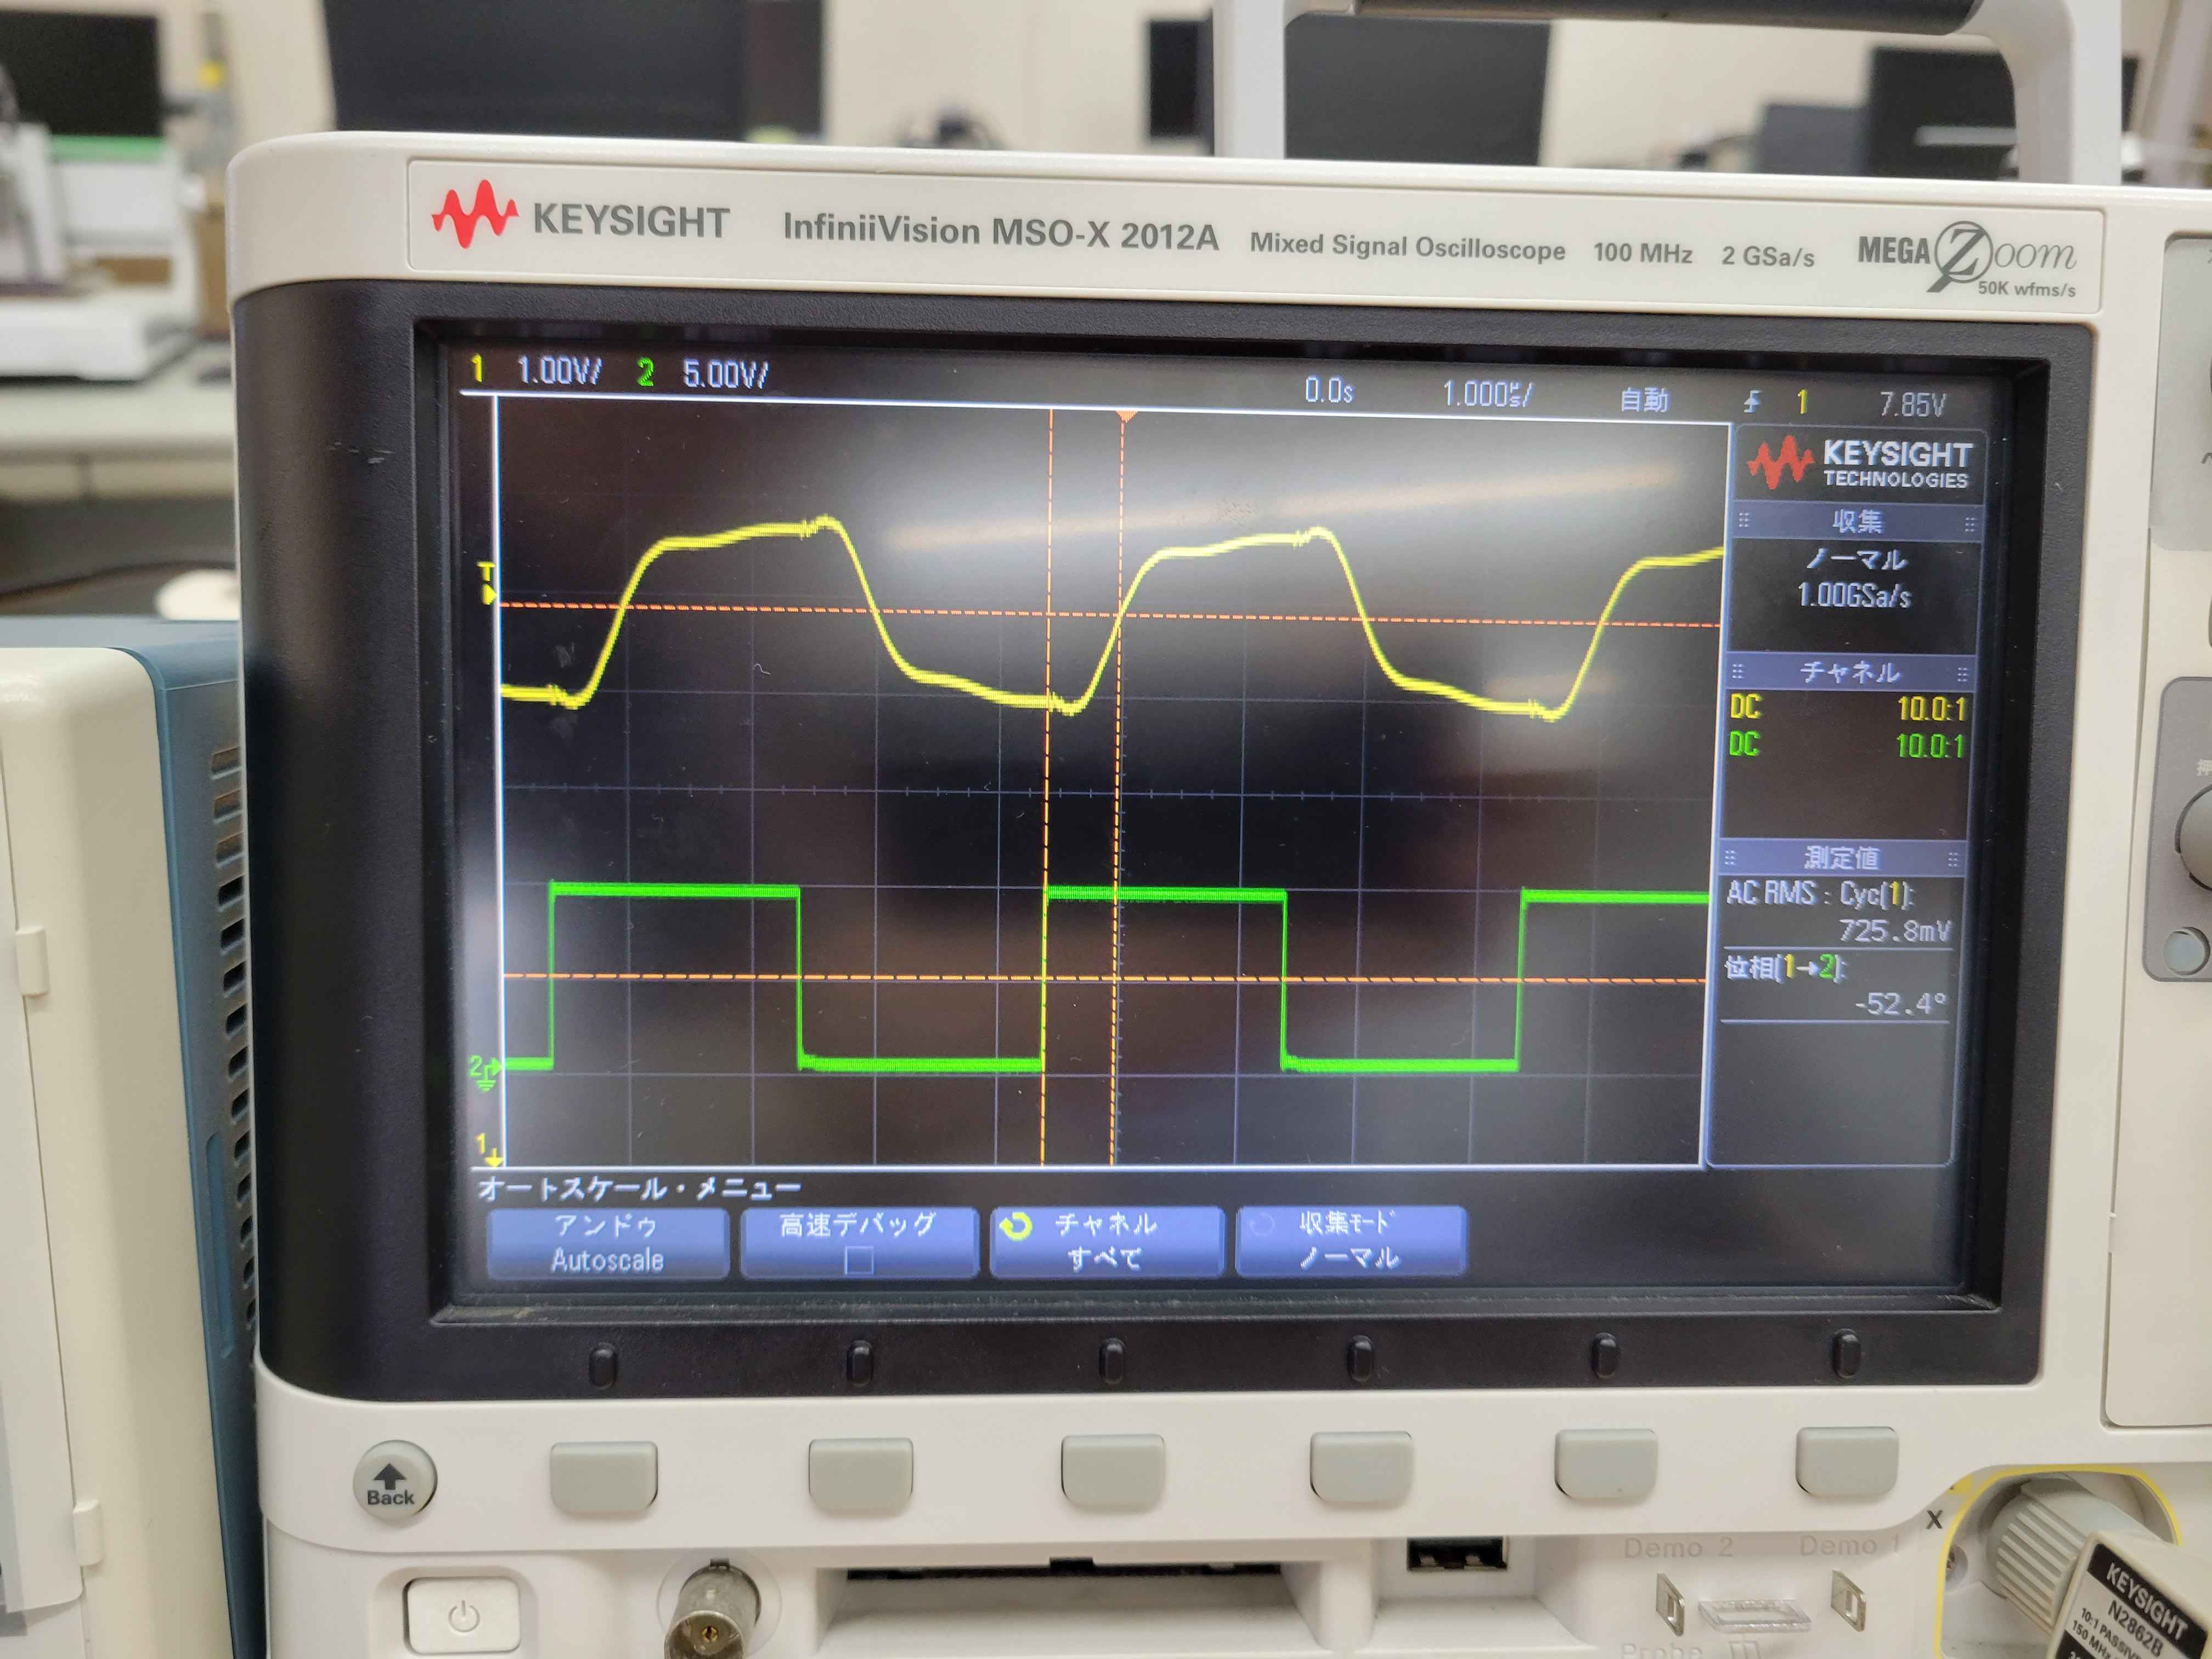
\includegraphics[width=0.4\textwidth]{fig/250.jpg}
      \caption{j250 kHzの信号でLEDを光らせた時の波形}
      \label{jukou3}
      \end{figure}
      入力波形に対応して出力の波形が変化していることを確認できた。
      フィルタを通すことで、受講部の出力をより明確にすることを目標にしたいと思う。
\end{multicols}

\end{document}